\documentclass{article}

\usepackage{fancyhdr}
\usepackage[parfill]{parskip}
\usepackage{tikz}

\pagestyle{fancyplain}

\author{Todd Davies}
\title{3.2.7 Transport in organisms}
\date{\today}

\begin{document}

\rhead{3.2.7 Transport in organisms}
\lhead{\today}

\maketitle

\section*{Surface area to mass ratio}
\thispagestyle{empty}

Every organism must exchange substances with their environment. Many cells need
oxygen, and produce waste products such as carbon dioxide. Lots of organisms
must keep their body temperature within certain bounds too.

Small animals have a high surface area to volume ratio. Larger animals have a
smaller surface to area ratio. If you're stuck, just compare the volume and
surface areas of two cubes.

\section*{Exchange organs and mass transport systems}

All organisms need to supply all of their cells with the right
nutrients and ensure that there is no build up of waste products in cells.

Different organisms do this differently:

\begin{itemize}

	\item {\bf Single celled organisms} can usually rely on diffusion to
	transport substances. The rate of diffusion is fast enough (since the
	organism is very small) that the organism doesn't need a specialised
	transport mechanism.

	\item {\bf Multicellular organisms} can't rely on diffusion of substances
	for the following reasons:

		\begin{itemize}

			\item Some cells are deep within the body, far from the environment
			where the substances need to come from/go to.

			\item Large animals have a very low surface area to mass ratio and
			so they wouldn't be able to exchange enough substances using such a
			proportionally small surface area.

		\end{itemize}

	Concequently, multicellular organisms rely on mass transport systems such as
	the circulatory system in mammals to transport substances and specialised
	exchange organs such as lungs or gills in order to exchange substances with
	the environment efficiently.

\end{itemize}

\section*{Heat exchange and body shape}

The rate of heat loss is higher in small organisms, since they have a larger
surface area to mass ratio. The opposite is true for large animals, since they
have lots of respiring, heat producing cells in the middle of their bodies and
relatively little surface area with which to lose the heat.

Animals with a compact shape have little surface area with which to lose heat.
Animals with lots of flaps and folds have a larger surface area and usually lose
heat faster.

Organisms are adapted to their environment, they are a specific shapes or
behaviours that help them to survive in their climate. Examples include:

\begin{itemize}

	\item Hot environments usually have small animals living there, they can
	lose their heat quickly. They often have adapted kidneys to produce less
	urine so they have to lose less water.

	\item If a small animal is in a cold region, it often has a very high
	metabolic rate to compensate. Theis can also be accompanied by lots of fur
	and small ears and legs to reduce the surface area.

	\item Animals living in hot regions often have large legs, saggy skin and
	flappy ears (e.g. elephants) in order to maximise their surface area so
	they can lose heat easily.

\end{itemize}

\section*{Gas exchange}

Gas exchange surfaces usually have two major adaptations; a large surface area
and a very short diffusion pathway (i.e. they're thin). Often, a mass transport
system is used in conjunction with the gas exchange surface in order to keep the
concentration gradient steep and ensure diffusion happens as fast as possible.

Single celled organisms are able to have gases diffuse through their outer
surface. They can do this since the diffusion pathway is very short (often just
the plasma membrane) and they have a very high surface area to mass ratio.

\subsection*{Fish}

Fish use gas exchange systems even though they live underwater.
They use a counter-current system to get the most oxygen they can. It involves
the following stages:

\begin{enumerate}

	\item Water (containing oxygen) enters the mouth of the fish as it swims
	(yes, there is a reason fish always look so gormless).

	\item The water then enters the gills. Each gill is made of small plates
	called gill filaments which give a large surface area.

	\item Each gill filament has lots of lamellae on (little arcs of tissue
	rising from the gill filament). The lamellae increase the total surface
	area of the gills.

	\item The lamellae have lots of capillaries with a short diffusion pathway
	that speeds up diffusion.

	\item Blood flows through the lamellae in the opposite direction to the flow
	of water, meaning that there is always a large concentration gradient
	between the water and the blood and the maxiumum amount of oxygen diffuses
	in.

\end{enumerate}

\subsection*{Insects}

Insects use tracheae to exchange gases. Tracheae are microscopic air-filled
pipes, into which air diffues via spiracles. Oxygen travels down a concentration
gradient towards cells and carbon dioxide goes in the opposite direction towards
the spiracles in order to be released into the atmosphere.

The tracheae branch off into smaller tracheoles which have very thin permeable
walls and go to individial cells. Insects use rhythmic abdominal movements to
transport air into and out of the spiracles.

Insects have a waxy body, hairs around their spiracles and can shut their
spiracles. All of these factors help the insect conserve water if it is becoming
dehydrated.

\subsection*{Plants}

The main gas exchange surface on plants is the surface of the mesophyll cells in
the leaf. They're well adapted for their function and have a large surface area.
The measophyll cells are actually inside the leaf, gasses move in and out of the
pores in surface of the leaf called the stomata.

The stomata are able to open and close depending on whether the plant needs to
exchange gasses, or if it needs to conserve water. Guard cells control the
opening and closing of the stomata by becoming turgid in or flacid depending on
whether the stomata needs to be closed (turgid) or open (flacid).

\section*{Mass transport systems}

Multicellular organisms need a system to efficiently transport nutrients around
their bodies. This often comes in the form of a circulatory system.

In many organisms, a heart punps blood around the body though blood vessels. The
names of the blood vessels that go to the heart, liver and kidneys need to be
learnt. Blood transports lots of useful substances around the body, including
oxygen, carbon dioxide, products of digestion, hormones and  many other things.

There are two circuits of blood around the body. One goes from the heart to the
lungs, the other from the heart around the rest of the body. The heart has it's
own blood supply (part of the latter circuit).

\begin{center}
	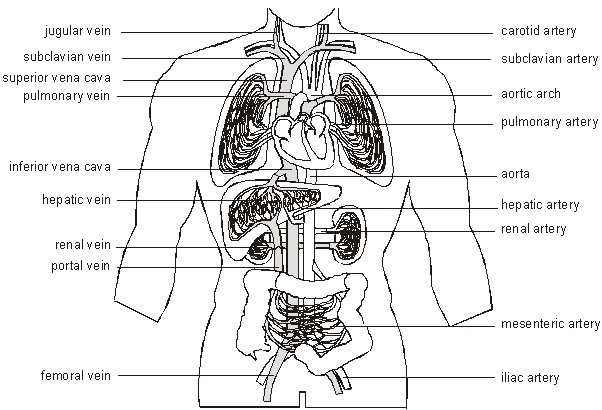
\includegraphics[scale=0.6]{circulatory_system}
\end{center}

\subsection*{Types of blood vessels}

There are three types of blood vessels; vrteries, veins and capillaries.

\subsubsection*{Arteries}

Arteries carry blood from the heart to the rest of the body. They have thick,
muscular walls with elastic tissue so that they can cope with the high pressure
produced by heartbeats. The inner lining is folded to allow for expansion.

Arteries divide into smaller vessels called arterioles. Blood can be directed to
different parts of the body by the muscular walls in the arterioles contracting
in order to restrict blood flow (for example to decrease the rate of digestion
during excersise).

\subsubsection*{Veins}

Veins take blood from the heart and are under low pressure. They have a wider
lumen than arteries with little elastic or muscular tissue. Veins contain valves
to stop blood from flowing backwards, and blood flow is often assisted by the
contraction of body muscles around them.

\subsubsection*{Capillaries}

Capillaries are the smallest blood vessels. Substances that are being
transported in the blood are exchanged through the thin (one cell thick)
capillary membrane seperating blood from the cells. The diffusion pathway is
very short; capillaries are adapted for diffusion.

\subsection*{Tissue fluid}

Tissue fluid is the fluid that surround cells. It is made from substances that
have left the blood via capillaries such as water, oxygen and nutrients. Cells
absorb nutrients and deposit waste there.

Tissue fluid moves out of the capillaries by pressure filtration, which involves
the following steps:

\begin{itemize}

	\item At the start of the capillary, the pressure is high, and fluid is
	forced out of the capillary into spaces around the cells.

	\item As fluid leaves the capillary, the pressure drops, so that when the
	capillary nears a vein, the pressure is low.

	\item Due to the low pressure here, water re-enters the capillary by
	osmisis. This restores the pressure in the capillary.

\end{itemize}

Note that no large proteins or red blood cells are present in the tissue fluid -
they can't diffuese through the membrane of the capillary. If they do get out,
they are drained into the lymph system which transports them back into the blood
stream.

\section*{Water transport in plants}

\subsection*{Through the roots}

Water enters the plant through root hair cells. The hairs on the cell increase
its surface area, so that it can take up water faster. In order to enter the
plant, the water must flow through the cortex and endodermis before finally
entering the xylem.

Water can take two routes through the root; the symplastic and apoplastic
pathways.

\subsubsection*{Symplast pathway}

The symplast pathway goes through the cytoplasm (living parts) of cells to reach it's
destination. It goes between cells via plasmodesmata (small gaps in the cell
walls).

\subsubsection*{Apoplast pathway}

The apoplast pathway goes through the cell walls (non living parts of the cell).
The cell walls are very absorbent and water can simply diffuse through them.

When the apoplastic pathway reaches the endodermis cells though, its path is
blocked by a waxy strip called the {\bf Casparian strip}. This forces the water
to take the symplast pathway so that the plant can better control how much water
is entering the plant (too much would be bad).

The main pathway that is used is the apoplastic pathway, since that has the
least resistance.

\subsection*{The cohesion tension theory}

The cohesion tension theory helps explain why the water flows against gravity up
the stem of the plant. Since water evaporates from the leaves (at the top of the
stem) a tension is created in the leaf which pulls more water into the leaf.

Water molecules are cohesive, and so when some are pulled into the leaf, others
follow, and more follow them. This means that the whole column of water in the
xylem moves up the plant towards the leaves.

\subsection*{Root pressure}

Another way that water is moved up the stem is root pressure. When water is
transported into the plant from the roots, the pressure at the bottom of the
plant increases, forcing water up the stem. This is only a weak force, but it is
vital in small plants before the leaves are fully developed.

\subsection*{Transpiration}

Transpiration is the loss of water from a plants surface. Water evaporates from
the moist cell walls and accumilates in the spongy mesophyll. When the stomata
are open, water then moves out of the plant along a concentration gradient.

There are four factors affecting the rate of transpiration:

\begin{itemize}

    \item {\bf Light} - the stomata open with light (to allow gas exchange), so
	more water escapes.

	\item {\bf Temperature} - water molecules have a higher energy at higher
	temperatures, and so evaporate more easily, increasing the rate of
	transpiration.

	\item {\bf Humidity} - dry climates with a low humidity increases the
	concentration gradient between the leaf and the air and more water
	evaporates.

	\item {\bf Wind} - the windier it is, the faster the rate of transpiration,
	since lots of air blows away the water on the leaf which increases the
	concentration gradient and rate of transpiration further.

\end{itemize}

\end{document}